%==============================================================================
% tento soubor pouzijte jako zaklad
% this file should be used as a base for the thesis
% Autoři / Authors: 2008 Michal Bidlo, 2019 Jaroslav Dytrych
% Kontakt pro dotazy a připomínky: sablona@fit.vutbr.cz
% Contact for questions and comments: sablona@fit.vutbr.cz
%==============================================================================
% kodovani: UTF-8 (zmena prikazem iconv, recode nebo cstocs)
% encoding: UTF-8 (you can change it by command iconv, recode or cstocs)
%------------------------------------------------------------------------------
% zpracování / processing: make, make pdf, make clean
%==============================================================================
% Soubory, které je nutné upravit nebo smazat: / Files which have to be edited or deleted:
%   projekt-20-literatura-bibliography.bib - literatura / bibliography
%   projekt-01-kapitoly-chapters.tex - obsah práce / the thesis content
%   projekt-01-kapitoly-chapters-en.tex - obsah práce v angličtině / the thesis content in English
%   projekt-30-prilohy-appendices.tex - přílohy / appendices
%   projekt-30-prilohy-appendices-en.tex - přílohy v angličtině / appendices in English
%==============================================================================
%\documentclass[slovak,zadani]{fitthesis} % bez zadání - pro začátek práce, aby nebyl problém s překladem
%\documentclass[english]{fitthesis} % without assignment - for the work start to avoid compilation problem
%\documentclass[zadani]{fitthesis} % odevzdani do wisu a/nebo tisk s barevnými odkazy - odkazy jsou barevné
%\documentclass[english,zadani]{fitthesis} % for submission to the IS FIT and/or print with color links - links are color
%\documentclass[zadani,print]{fitthesis} % pro černobílý tisk - odkazy jsou černé
%\documentclass[english,zadani,print]{fitthesis} % for the black and white print - links are black
\documentclass[slovak]{fitthesis} % pro barevný tisk - odkazy jsou černé, znak VUT barevný
%\documentclass[english,zadani,cprint]{fitthesis} % for the print - links are black, logo is color
% * Je-li práce psaná v anglickém jazyce, je zapotřebí u třídy použít 
%   parametr english následovně:
%   If thesis is written in English, it is necessary to use 
%   parameter english as follows:
%      \documentclass[english]{fitthesis}
% * Je-li práce psaná ve slovenském jazyce, je zapotřebí u třídy použít 
%   parametr slovak následovně:
%   If the work is written in the Slovak language, it is necessary 
%   to use parameter slovak as follows:
%      \documentclass[slovak]{fitthesis}
% * Je-li práce psaná v anglickém jazyce se slovenským abstraktem apod., 
%   je zapotřebí u třídy použít parametry english a enslovak následovně:
%   If the work is written in English with the Slovak abstract, etc., 
%   it is necessary to use parameters english and enslovak as follows:
%      \documentclass[english,enslovak]{fitthesis}

% Základní balíčky jsou dole v souboru šablony fitthesis.cls
% Basic packages are at the bottom of template file fitthesis.cls
% zde můžeme vložit vlastní balíčky / you can place own packages here

% Kompilace po částech (rychlejší, ale v náhledu nemusí být vše aktuální)
% Compilation piecewise (faster, but not all parts in preview will be up-to-date)
% \usepackage{subfiles}

% Nastavení cesty k obrázkům
% Setting of a path to the pictures
%\graphicspath{{obrazky-figures/}{./obrazky-figures/}}
%\graphicspath{{obrazky-figures/}{../obrazky-figures/}}

%---rm---------------
\renewcommand{\rmdefault}{lmr}%zavede Latin Modern Roman jako rm / set Latin Modern Roman as rm
%---sf---------------
\renewcommand{\sfdefault}{qhv}%zavede TeX Gyre Heros jako sf
%---tt------------
\renewcommand{\ttdefault}{lmtt}% zavede Latin Modern tt jako tt

% vypne funkci šablony, která automaticky nahrazuje uvozovky,
% aby nebyly prováděny nevhodné náhrady v popisech API apod.
% disables function of the template which replaces quotation marks
% to avoid unnecessary replacements in the API descriptions etc.
\csdoublequotesoff

\usepackage{pdfpages}
\usepackage{svg}
\usepackage{amsmath}
\usepackage{url}
\usepackage{graphicx,wrapfig,lipsum}
\usepackage{minted}
\usepackage{textcomp}
\usepackage{siunitx}
\usepackage[utf8]{inputenc}
\DeclareUnicodeCharacter{2190}\leftarrow % ←

\definecolor{bluekeywords}{rgb}{0,0,1}
\definecolor{greencomments}{rgb}{0,0.5,0}
\definecolor{redstrings}{rgb}{0.64,0.08,0.08}
\definecolor{xmlcomments}{rgb}{0.5,0.5,0.5}
\definecolor{types}{rgb}{0.17,0.57,0.68}

\usepackage{listings}
\lstset{language=[Sharp]C,
captionpos=b,
%numbers=left, %Nummerierung
%numberstyle=\tiny, % kleine Zeilennummern
frame=lines, % Oberhalb und unterhalb des Listings ist eine Linie
showspaces=false,
showtabs=false,
breaklines=true,
showstringspaces=false,
breakatwhitespace=true,
escapeinside={(*@}{@*)},
commentstyle=\color{greencomments},
morekeywords={partial, var, value, get, set},
keywordstyle=\color{bluekeywords},
stringstyle=\color{redstrings},
basicstyle=\ttfamily\small,
}

% =======================================================================
% balíček "hyperref" vytváří klikací odkazy v pdf, pokud tedy použijeme pdflatex
% problém je, že balíček hyperref musí být uveden jako poslední, takže nemůže
% být v šabloně
% "hyperref" package create clickable links in pdf if you are using pdflatex.
% Problem is that this package have to be introduced as the last one so it 
% can not be placed in the template file.
\ifWis
\ifx\pdfoutput\undefined % nejedeme pod pdflatexem / we are not using pdflatex
\else
  \usepackage{color}
  \usepackage[unicode,colorlinks,hyperindex,plainpages=false,pdftex]{hyperref}
  \definecolor{hrcolor-ref}{RGB}{223,52,30}
  \definecolor{hrcolor-cite}{HTML}{2F8F00}
  \definecolor{hrcolor-urls}{HTML}{092EAB}
  \hypersetup{
	linkcolor=hrcolor-ref,
	citecolor=hrcolor-cite,
	filecolor=magenta,
	urlcolor=hrcolor-urls
  }
  \def\pdfBorderAttrs{/Border [0 0 0] }  % bez okrajů kolem odkazů / without margins around links
  \pdfcompresslevel=9
\fi
\else % pro tisk budou odkazy, na které se dá klikat, černé / for the print clickable links will be black
\ifx\pdfoutput\undefined % nejedeme pod pdflatexem / we are not using pdflatex
\else
  \usepackage{color}
  \usepackage[unicode,colorlinks,hyperindex,plainpages=false,pdftex,urlcolor=black,linkcolor=black,citecolor=black]{hyperref}
  \definecolor{links}{rgb}{0,0,0}
  \definecolor{anchors}{rgb}{0,0,0}
  \def\AnchorColor{anchors}
  \def\LinkColor{links}
  \def\pdfBorderAttrs{/Border [0 0 0] } % bez okrajů kolem odkazů / without margins around links
  \pdfcompresslevel=9
\fi
\fi
% Řešení problému, kdy klikací odkazy na obrázky vedou za obrázek
% This solves the problems with links which leads after the picture
\usepackage[all]{hypcap}

% Informace o práci/projektu / Information about the thesis
%---------------------------------------------------------------------------
\projectinfo{
  %Prace / Thesis
  project={DP},            %typ práce BP/SP/DP/DR  / thesis type (SP = term project)
  year={2023},             % rok odevzdání / year of submission
  date=\today,             % datum odevzdání / submission date
  %Nazev prace / thesis title
  title.cs={Analýza a vizualizace dat z úředních desek města Brna},  % název práce v češtině či slovenštině (dle zadání) / thesis title in czech language (according to assignment)
  title.en={Analysis and visualization OF Brno's official notice boards}, % název práce v angličtině / thesis title in english
  %title.length={14.5cm}, % nastavení délky bloku s titulkem pro úpravu zalomení řádku (lze definovat zde nebo níže) / setting the length of a block with a thesis title for adjusting a line break (can be defined here or below)
  %sectitle.length={14.5cm}, % nastavení délky bloku s druhým titulkem pro úpravu zalomení řádku (lze definovat zde nebo níže) / setting the length of a block with a second thesis title for adjusting a line break (can be defined here or below)
  %dectitle.length={14.5cm}, % nastavení délky bloku s titulkem nad prohlášením pro úpravu zalomení řádku (lze definovat zde nebo níže) / setting the length of a block with a thesis title above declaration for adjusting a line break (can be defined here or below)
  %Autor / Author
  author.name={Matej},   % jméno autora / author name
  author.surname={Mištík},   % příjmení autora / author surname 
  author.title.p={Bc.}, % titul před jménem (nepovinné) / title before the name (optional)
  %author.title.a={Ph.D.}, % titul za jménem (nepovinné) / title after the name (optional)
  %Ustav / Department
  department={UIFS}, % doplňte příslušnou zkratku dle ústavu na zadání: UPSY/UIFS/UITS/UPGM / fill in appropriate abbreviation of the department according to assignment: UPSY/UIFS/UITS/UPGM
  % Školitel / supervisor
  supervisor.name={Jiří},   % jméno školitele / supervisor name 
  supervisor.surname={Hynek},   % příjmení školitele / supervisor surname
  supervisor.title.p={Ing.},
  supervisor.title.a={Ph.D.},%titul před jménem (nepovinné) / title before the name (optional)
  %supervisor.title.a={},    %titul za jménem (nepovinné) / title after the name (optional)
  % Klíčová slova / keywords
  keywords.cs={Uřední deska, edeska, vizualizace, Brno, HTML, JSON}, % klíčová slova v českém či slovenském jazyce / keywords in czech or slovak language
  keywords.en={Official notice board, eboard, visualization, Brno, HTML, JSON}, % klíčová slova v anglickém jazyce / keywords in english
  %keywords.en={Here, individual keywords separated by commas will be written in English.},
  % Abstrakt / Abstract
  abstract.cs={Cieľom tejto práce bolo analyzovať, prepojiť, zobraziť a použiť dáta samostatných častí mesta Brna. Práca sa zamerala na využitie lokácii jednotlivých úradných dosiek a ich prepojením s používateľom. Vytvorená aplikácia dovoľuje používateľovi zobraziť úradne dosky v jeho blízkosti. Prínosom tejto práce je nový spôsob notifikácii úradných dosiek, ktoré sa presunú z fyzického do virtuálneho prostredia.}, % abstrakt v českém či slovenském jazyce / abstract in czech or slovak language
  abstract.en={The goal of this thesis is to analyze, integrate and visualize and use the data of urban territories of Brno.}, % abstrakt v anglickém jazyce / abstract in english
  %abstract.en={An abstract of the work in English will be written in this paragraph.},
  % Prohlášení (u anglicky psané práce anglicky, u slovensky psané práce slovensky) / Declaration (for thesis in english should be in english)
  declaration={Prehlasujem, že som túto diplomovú prácu vypracoval samostatne pod vedením pána Ing. Jiřího Hynka.
Uviedol som všetky literárne pramene, publikácie a ďalšie zdroje, z ktorých
som čerpal.},
  %declaration={I hereby declare that this Bachelor's thesis was prepared as an original work by the author under the supervision of Mr. X
% The supplementary information was provided by Mr. Y
% I have listed all the literary sources, publications and other sources, which were used during the preparation of this thesis.},
  % Poděkování (nepovinné, nejlépe v jazyce práce) / Acknowledgement (optional, ideally in the language of the thesis)
  acknowledgment={Chcel by som poďakovať môjmu vedúcemu práce Jiřímu Hynkovi a takisto Kristíne Záklovej za spoluprácu pri získavaní zdrojov a konzultovaní práce.},
  %acknowledgment={Here it is possible to express thanks to the supervisor and to the people which provided professional help
%(external submitter, consultant, etc.).},
  % Rozšířený abstrakt (cca 3 normostrany) - lze definovat zde nebo níže / Extended abstract (approximately 3 standard pages) - can be defined here or below
  %extendedabstract={Do tohoto odstavce bude zapsán rozšířený výtah (abstrakt) práce v českém (slovenském) jazyce.},
  %extabstract.odd={true}, % Začít rozšířený abstrakt na liché stránce? / Should extended abstract start on the odd page?
  %faculty={FIT}, % FIT/FEKT/FSI/FA/FCH/FP/FAST/FAVU/USI/DEF
  faculty.cs={Fakulta informačních technologií}, % Fakulta v češtině - pro využití této položky výše zvolte fakultu DEF / Faculty in Czech - for use of this entry select DEF above
  faculty.en={Faculty of Information Technology}, % Fakulta v angličtině - pro využití této položky výše zvolte fakultu DEF / Faculty in English - for use of this entry select DEF above
  department.cs={Ústav matematiky}, % Ústav v češtině - pro využití této položky výše zvolte ústav DEF nebo jej zakomentujte / Department in Czech - for use of this entry select DEF above or comment it out
  department.en={Institute of Mathematics} % Ústav v angličtině - pro využití této položky výše zvolte ústav DEF nebo jej zakomentujte / Department in English - for use of this entry select DEF above or comment it out
}

% Rozšířený abstrakt (cca 3 normostrany) - lze definovat zde nebo výše / Extended abstract (approximately 3 standard pages) - can be defined here or above
%\extendedabstract{Do tohoto odstavce bude zapsán výtah (abstrakt) práce v českém (slovenském) jazyce.}
% Začít rozšířený abstrakt na liché stránce? / Should extended abstract start on the odd page?
%\extabstractodd{true}

% nastavení délky bloku s titulkem pro úpravu zalomení řádku - lze definovat zde nebo výše / setting the length of a block with a thesis title for adjusting a line break - can be defined here or above
%\titlelength{14.5cm}
% nastavení délky bloku s druhým titulkem pro úpravu zalomení řádku - lze definovat zde nebo výše / setting the length of a block with a second thesis title for adjusting a line break - can be defined here or above
%\sectitlelength{14.5cm}
% nastavení délky bloku s titulkem nad prohlášením pro úpravu zalomení řádku - lze definovat zde nebo výše / setting the length of a block with a thesis title above declaration for adjusting a line break - can be defined here or above
%\dectitlelength{14.5cm}

% řeší první/poslední řádek odstavce na předchozí/následující stránce
% solves first/last row of the paragraph on the previous/next page
\clubpenalty=10000
\widowpenalty=10000

% checklist
\newlist{checklist}{itemize}{1}
\setlist[checklist]{label=$\square$}

% Nechcete-li, aby se u oboustranného tisku roztahovaly mezery pro zaplnění stránky, odkomentujte následující řádek / If you do not want enlarged spacing for filling of the pages in case of duplex printing, uncomment the following line
% \raggedbottom

\begin{document}
  % Vysazeni titulnich stran / Typesetting of the title pages
  % ----------------------------------------------
  \maketitle
  % Obsah
  % ----------------------------------------------
  \setlength{\parskip}{0pt}
  \setcounter{tocdepth}{1}  
  {\hypersetup{hidelinks}\tableofcontents}
  
  % Seznam obrazku a tabulek (pokud prace obsahuje velke mnozstvi obrazku, tak se to hodi)
  % List of figures and list of tables (if the thesis contains a lot of pictures, it is good)
  \ifczech
    \renewcommand\listfigurename{Seznam obrázků}
  \fi
  \ifslovak
    \renewcommand\listfigurename{Zoznam obrázkov}
  \fi
  % {\hypersetup{hidelinks}\listoffigures}
  
  \ifczech
    \renewcommand\listtablename{Seznam tabulek}
  \fi
  \ifslovak
    \renewcommand\listtablename{Zoznam tabuliek}
  \fi
  % {\hypersetup{hidelinks}\listoftables}

  \ifODSAZ
    \setlength{\parskip}{0.5\bigskipamount}
  \else
    \setlength{\parskip}{0pt}
  \fi

  % vynechani stranky v oboustrannem rezimu
  % Skip the page in the two-sided mode
  \iftwoside
    \cleardoublepage
  \fi

  % Text prace / Thesis text
  % ----------------------------------------------
  \ifenglish
    \input{projekt-01-kapitoly-chapters-en}
  \else
    % Tento soubor nahraďte vlastním souborem s obsahem práce.
%=========================================================================
% Autoři: Michal Bidlo, Bohuslav Křena, Jaroslav Dytrych, Petr Veigend a Adam Herout 2019
\chapter{Úvod}

Aktuálna doba či už v závislosti od Pandémie alebo digitalizácie naučila občanov ostávať vo svojich obydliach, zatiaľ čo úradné oznamy sú buď zobrazené v neprehľadných formách na internetových stránkach alebo fyzicky na úradoch mesta.

Ich centralizácia a digitálne sprehľadnenie je nevyhnutné pre jednoduchú komunikáciu úradu a obyvateľa mestskej časti. Úlohami práce je preto integrácia dátových sád 29 častí mesta Brna, využitie geografickej polohy jednotlivých úradných dosiek a ich prepojení s obyvateľstvom.

V Teórii \ref{theory} sa práca zameriava na existujúce riešenia a stav aktuálnych poskytnutých dát.

\chapter{Teória}
\label{theory}
Táto kapitola opisuje, aké boli aktuálne riešenia ustanovenie pevnej formy dát, ich zjednotenie a následné informovanie užívateľov pomocou mobilných aplikácii.


\section{Riešenie digitalizácie úradných dosiek}

Digitálne dosky od sprostredkovateľa obec24, GROUP24 INNOVATIONS s.r.o., ktorá ponúka digitalizáciu úradných dosiek pomocou veľkoplošných obrazoviek s dotykovým displejom, pre jednoduchú navigáciu a interakciu. Takáto digitalizácia urýchľuje vystavovanie, dovoľuje rýchlym úpravám, škálovateľnosti atď. Avšak riešenia sú ponúkané a lokalizované na mestských úradom čím sa otázka dostupnosti bohužiaľ nevyriešila. Jedno z riešení Obce24 je na obrázku \ref{urednideskaobec24}.


\begin{figure}[H]
	\centering
	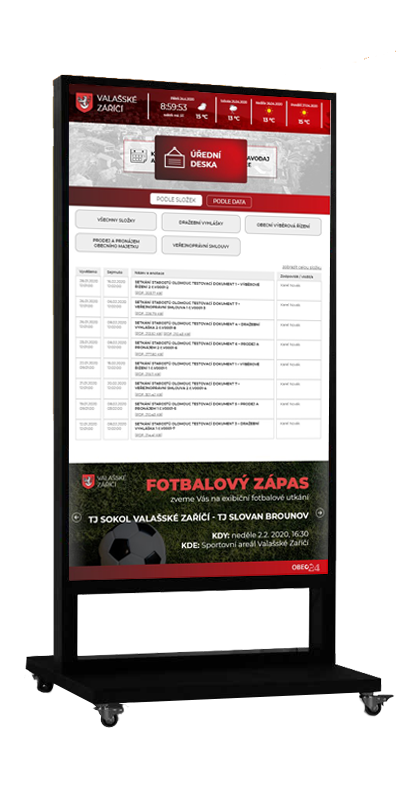
\includegraphics[width=0.25 \linewidth]{img/urednideskaobec24.png}
	\caption{MODEL i01 INDOOR
SAMOSTATNĚ STOJÍCÍ poskytujúci dotykovú obrazovku pre navigúciu v úradných doskách}
	\label{urednideskaobec24}
\end{figure}

\subsection{Notifikačná aplikácia}
Notifikácie sú prevedené pomocou aplikácie Telegram spojené s GitHub. Telegram je chatovacia služba. Je využitá z toho dôvodu, že dovoľuje jednoducho naprogramovať automatických botov, jeden už z existujúcich, ktorý umožňuje upozorniť na novo vykonanú zmenu v github projekte  \cite{notifikacniAplikace}. Notifikácia je zobrazená na obrázku 

\begin{figure}[H]
	\centering
	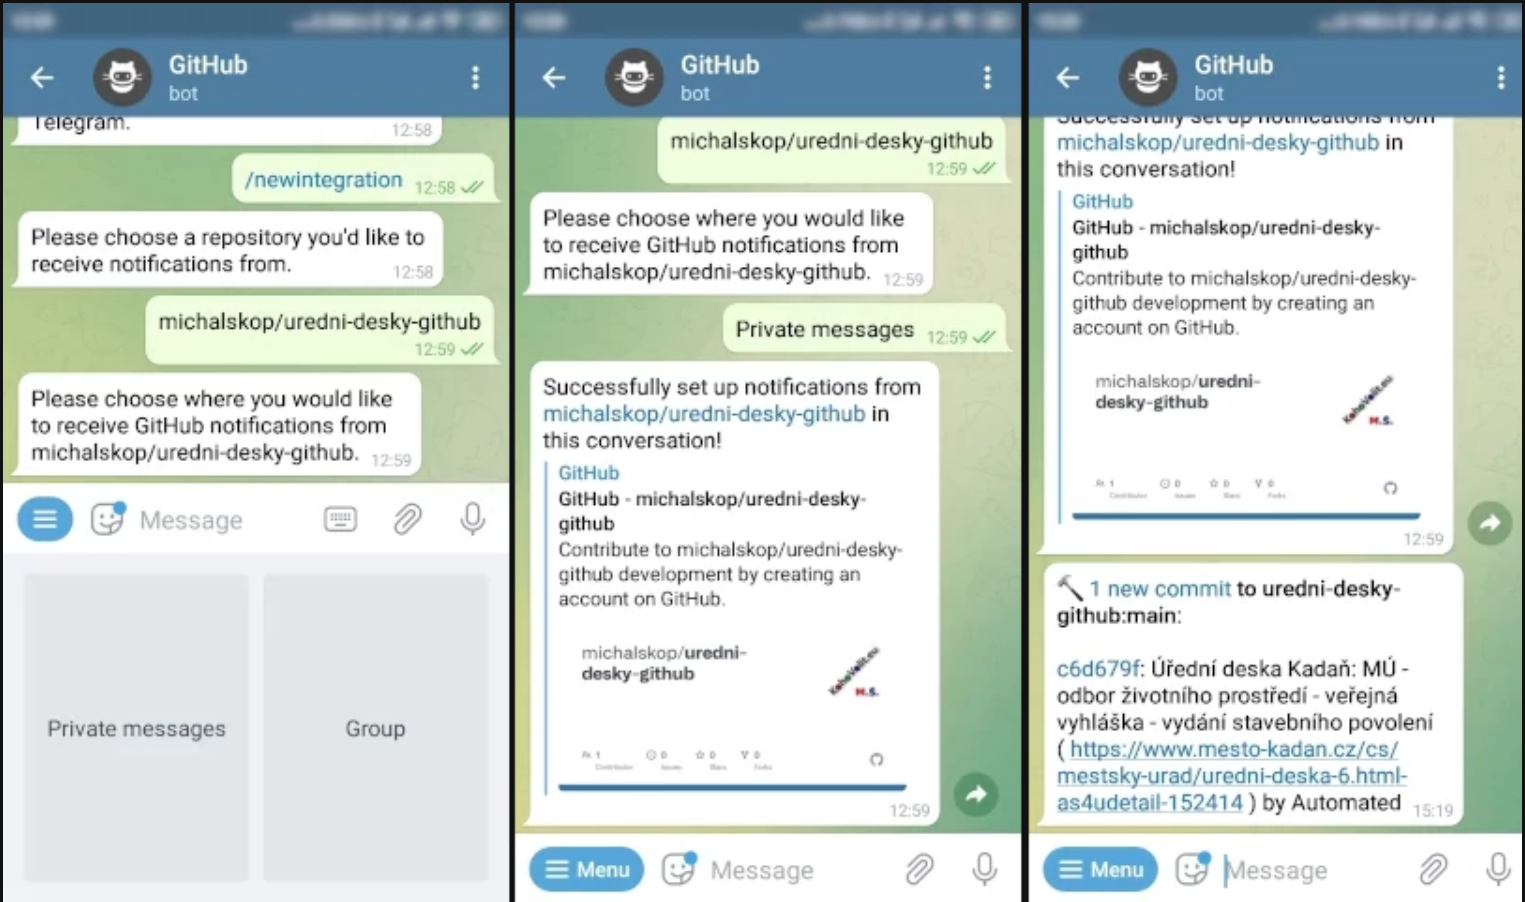
\includegraphics[width=0.85 \linewidth]{img/TelegramNotifikaceUredniDeska.png}
	\caption{Automatické upozornenie, ktoré príde ako textová správa do aplikácie telegram pri pridaní úradnej dosky}
	\label{TelegramNotifikaceUredniDeska}
\end{figure}

\noindent
Tento koncept sa môže použiť práve pri notifikácií obyvateľov, pri zmenách v ich okolí.



\subsection{Projekt edesky.cz}
Projekt edesky zhromažďuje úradné dosky v Českej Republike. Vrámci tohoto zjednotenia poskytuje aj úradne dosky každej mestskej časti Brna\footnote{\url{https://edesky.cz/dokumenty?action=index&controller=documents&hledat_stare=1&zdroj=104}}.


Projekt je tvorený jednotlivcom Marekom Aufartom. Projekt má verejnú dokumentáciu a poskytuje aj API pre vyhľadávanie dokumentov a jednotlivých úradných dosiek.

Aktualita dát má časovú odchýlku pridania na portál rádovo 1-2 hodiny od zverejnenia na oficiálnych stránkach mesta Brna.



%https://edesky.cz/dokumenty?action=index&controller=documents&hledat_stare=1&zdroj=104


\section{Datové sady mesta Brna}
EdeskaBrno - https://edeska.brno.cz/eDeska/



\subsection{Členenie Brna}


Zdroj desek mimo edeska od mesta brna: 

reckovice - \href{http://www.udeska.info/deska.php?login=reckovice}{Reckovice}
oresin - \href{https://www.brno-oresin.cz/uredni-deska.asp}{Oresin}
bystc - \href{https://www.bystrc.cz/uredni-deska.html}{Bystrc}
cervnovice - \href{https://www.cernov.cz/vismo/zobraz_dok.asp?id\_org=2052&id\_ktg=1003}{Cernovice} 

Brno chrlice nemá uredni desky

\href{https://www.mcivanovice.cz/uredni-deska}{Ivanovice}








\section{Otevřená Data}
Open data

\section{Otevřené formální normy}
Od 1.2.2022 je povinnosťou zverejňovať otvorenné dáta podle \cite{ofnUredeniDesky}



\chapter{Analýza}
\label{Analysis}
Táto kapitola sa zamiera na analýzu chybovosti dátových sád, dodržovanie noriem a pod.

\section{system zadavania edesiek}


\section{Analýza edesky.cz}
portál zhromažďuje úspešne 14 z 28 okresov poskytujúcich úradné dosky pre mesto Brno \href{https://edesky.cz/dokumenty?zdroj=104}{tu}. Ostatné dosky majú v svojej kategórii prázdny charakter a okresy Žebetín a Starý Lískovec nemá vo svojej databáze. Časť Brno-Slatina je priradená mimo mesta Brna.

\section{Analýza úradných dosiek podľa metskej časti}

Brno sa skladá z 29 metských častí, z toho dostupné otvorené dáta úradných dosiek sú v nasledujúcej tabuľke \ref{MestskeCastiDostupnost}:

\begin{table}[H]
    \centering
    \begin{tabular}{|l|l|l|l|l|l|}
    \hline
        Mestská časť & číslo & edeska Brno  & Edesky.cz & off. stránka  &  ONF \\ \hline
        Brno-Bohunice & & & \color{green}Áno & \href{https://www.brno-bohunice.cz/cs/urad-mestske-casti/uredni-deska.html}{Bohunice} & ~ \\ \hline
        Brno-Bosonohy & 24 & \color{green}Áno & \color{green}Áno & \href{https://edeska.brno.cz/eDeska24/}{Bosonohy} & ~ \\ \hline
        Brno-Bystrc & & & \color{green}Áno & \href{https://www.bystrc.cz/uredni-deska.html}{Bystrc} & ~\\ \hline
        Brno-Černovice & & & \color{green}Áno& \href{https://www.cernov.cz/vismo/zobraz_dok.asp?id\_org=2052&id\_ktg=1003}{Cernovice}  & ~ \\ \hline
        Brno-Chrlice & & \color{red}Nie& \color{red}Nie & \color{red}Nie & ~ \\ \hline
        Brno-Ivanovice & & & \color{red}Nie& \href{https://www.mcivanovice.cz/uredni-deska}{Ivanovice}& ~ \\ \hline
        Brno-Jehnice & & & \color{green}Áno & \href{http://brno-jehnice.cz/uredni-deska}{Jehnice}& ~ \\ \hline
        Brno-jih & 07 & \color{green}Áno & \color{red}Nie & \href{https://www.brno-jih.cz/uredni-deska/1}{Jih} & ~ \\ \hline
        Brno-Jundrov & & & \color{red}Nie& \href{https://www.jundrov.info/uredni-deska/2}{Jundrov} & ~ \\ \hline
        Brno-Kníničky & 14 & \color{green}Áno & \color{red}Nie & \href{https://edeska.brno.cz/eDeska14/}{Kníničky} &  ~ \\ \hline
        Brno-Kohoutovice & & & \color{red}Nie & \href{https://www.kohoutovice.brno.cz/uredni-deska/2}{Kohoutovice} & ~ \\ \hline
        Brno-Komín & & & \color{green}Áno & \href{https://www.brno-komin.cz/uredni-deska}{Komin}& ~ \\ \hline
        Brno-Královo Pole & 03 & \color{green}Áno & \color{red}Nie & \href{https://kralovopole.brno.cz/uredni-deska/2}{Krpole}& ~ \\ \hline
        Brno-Líšeň & & & \color{red}Nie & \href{https://www.brno-lisen.cz/elektronicka-uredni-deska/s1}{Lisen} & ~ \\ \hline
        Brno-Maloměřice a Obřany & & & \color{red}Nie & \href{https://www.malomerice.cz/uredni-deska/2}{MaO} & ~ \\ \hline
        Brno-Medlánky & 16 & \color{green}Áno & \color{green}Áno & \href{https://edeska.brno.cz//eDeska16/}{Medlanky} & ~ \\ \hline
        Brno-Nový Lískovec & & & \color{red}Nie & \href{https://www.novy-liskovec.cz/uredni-deska/2}{NLiskovec}  & ~ \\ \hline
        Brno-Ořešín & &  & \color{green}Áno & \href{https://www.brno-oresin.cz/uredni-deska.asp}{Oresin}& ~ \\ \hline
        Brno-Řečkovice a Mokrá Hora & & & \color{green}Áno & \href{http://www.udeska.info/deska.php?login=reckovice}{Reckovice}& ~ \\ \hline
        Brno-sever & 04 & \color{green}Áno & \color{red}Nie & \href{https://www.sever.brno.cz/uredni-deska.html}{Sever}& ~ \\ \hline
        Brno-Slatina & & & \color{green}Áno& \href{https://www.mcslatina.cz/uredni-deska}{Slatina} & ~ \\ \hline
        Brno-Starý Lískovec & & & \color{red}Nie & \href{https://www.staryliskovec.cz/cs/urad/uredni-deska-1.html}{SLiskovec} & ~ \\ \hline
        Brno-střed & 01 & \color{green}Áno & \color{red}Nie & \href{https://edeska.brno.cz/eDeska01/}{Stred} & ~ \\ \hline
        Brno-Tuřany & & & \color{green}Áno & \href{https://www.turany.cz/uredni-deska/}{Turany}& ~ \\ \hline
        Brno-Útěchov & & & \color{green}Áno & \href{https://brno-utechov.cz/category/uredni-deska/}{Utechov}& ~ \\ \hline
        Brno-Vinohrady & & & \color{green}Áno & \href{https://www.vinohrady.brno.cz/urad/uredni-deska}{Utechov} & ~ \\ \hline
        Brno-Žabovřesky & & & \color{red}Nie & \href{https://www.zabovresky.cz/uredni-deska/1}{Zabovresky} & ~ \\ \hline
        Brno-Žebětín & & & \color{green}Áno & \href{https://www.zebetin.cz/uredni-deska/2}{Zebetin} & ~ \\ \hline
        Brno-Židenice & 05 & \color{green}Áno & \color{red}Nie & \href{https://edeska.brno.cz/eDeska05/}{Zidenice}& ~ \\ \hline
    \end{tabular}
    \label{MestskeCastiDostupnost}
    \caption{Tabuľka zobrazuje dostupnosť jednotlivých zdrojov na podporovaných portáloch a ich zastúpnie v Otvorenej Normálnej Forme.}
\end{table}

\chapter{Návrh}
\label{Concept}

\chapter{Implementácia}

  \fi
  
  % Kompilace po částech (viz výše, nutno odkomentovat)
  % Compilation piecewise (see above, it is necessary to uncomment it)
  %\subfile{projekt-01-uvod-introduction}
  % ...
  %\subfile{chapters/projekt-05-conclusion}


  % Pouzita literatura / Bibliography
  % ----------------------------------------------
\ifslovak
  \makeatletter
  \def\@openbib@code{\addcontentsline{toc}{chapter}{Literatúra}}
  \makeatother
  \bibliographystyle{bib-styles/Pysny/skplain}
\else
  \ifczech
    \makeatletter
    \def\@openbib@code{\addcontentsline{toc}{chapter}{Literatura}}
    \makeatother
    \bibliographystyle{bib-styles/Pysny/czplain}
  \else 
    \makeatletter
    \def\@openbib@code{\addcontentsline{toc}{chapter}{Bibliography}}
    \makeatother
    \bibliographystyle{bib-styles/Pysny/enplain}
  %  \bibliographystyle{alpha}
  \fi
\fi
  \begin{flushleft}
  \bibliography{projekt-20-literatura-bibliography}
  \end{flushleft}

  % vynechani stranky v oboustrannem rezimu
  % Skip the page in the two-sided mode
  \iftwoside
    \cleardoublepage
  \fi

  % Prilohy / Appendices
  % ---------------------------------------------
  \appendix
\ifczech
  \renewcommand{\appendixpagename}{Přílohy}
  \renewcommand{\appendixtocname}{Přílohy}
  \renewcommand{\appendixname}{Příloha}
\fi
\ifslovak
  \renewcommand{\appendixpagename}{Prílohy}
  \renewcommand{\appendixtocname}{Prílohy}
  \renewcommand{\appendixname}{Príloha}
\fi
%  \appendixpage

% vynechani stranky v oboustrannem rezimu
% Skip the page in the two-sided mode
%\iftwoside
%  \cleardoublepage
%\fi
  
\ifslovak
%  \section*{Zoznam príloh}
%  \addcontentsline{toc}{section}{Zoznam príloh}
\else
  \ifczech
%    \section*{Seznam příloh}
%    \addcontentsline{toc}{section}{Seznam příloh}
  \else
%    \section*{List of Appendices}
%    \addcontentsline{toc}{section}{List of Appendices}
  \fi
\fi
  \startcontents[chapters]
  \setlength{\parskip}{0pt}
  % seznam příloh / list of appendices
  % \printcontents[chapters]{l}{0}{\setcounter{tocdepth}{2}}
  
  \ifODSAZ
    \setlength{\parskip}{0.5\bigskipamount}
  \else
    \setlength{\parskip}{0pt}
  \fi
  
  % vynechani stranky v oboustrannem rezimu
  \iftwoside
    \cleardoublepage
  \fi
  
  % Přílohy / Appendices
  \ifenglish
    \input{projekt-30-prilohy-appendices-en}
  \else
    \input{projekt-30-prilohy-appendices}
  \fi
  
  % Kompilace po částech (viz výše, nutno odkomentovat)
  % Compilation piecewise (see above, it is necessary to uncomment it)
  %\subfile{projekt-30-prilohy-appendices}
  
\end{document}
